\section{Large Scan}
Note: The analysis of this scan was later assumed to be incorrect, as it was found that the finesse is actually much higher. See more in section 5.
\subsubsection*{Settings}
Used settings:  \\
$f = 6.0$ Hz,  \\
Amplitude: 4.4 V,  \\
Offset: 370 mV.  \\
Filename: \texttt{ALL0002.CSV}.  


With these settings, the cavity presumably scanned over two FSRs.

\subsection{Full Trace}
Figure~\ref{fig:full} shows the full photodiode voltage (left axis) and the
sync voltage (right axis) as a function of time. The highlighted region
indicates the section of the data that was selected for further analysis (For comparison between sync voltage and piezo voltage, see Fig. \ref{fig:osci}).

\begin{figure}[H]
    \centering
    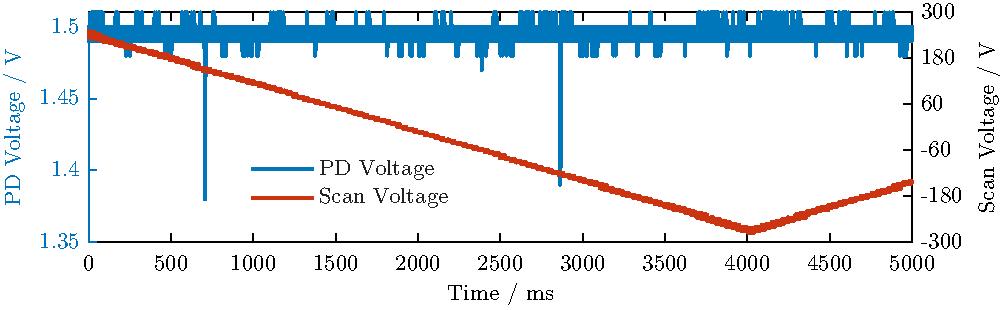
\includegraphics[width=\textwidth]{Figure_1.pdf}
    \caption{The rectangular signal is the sync signal of the function generator. The shaded region marks one ramp of the piezo (either increasing or decreasing the cavity length).}
    \label{fig:full}
\end{figure}

\subsection{Considered Region}
Figure~\ref{fig:fit} shows the selected region of the PD signal, normalized and
plotted with an Airy function. (This corresponds to Ramp 1 from the full trace.)

\begin{figure}[H]
    \centering
    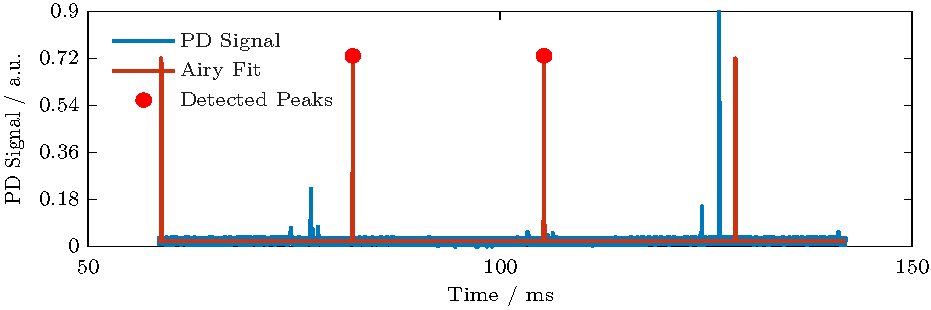
\includegraphics[width=\textwidth]{Figure_2.pdf}
    \caption{The two detected peaks lie directly underneath the fitted Airy function. The right-most peak is not well fitted, most likely due to non-linearity of the piezo scan.}
    \label{fig:fit}
\end{figure}

\subsection{Individual Peaks}
Each detected peak is shown separately in Figures~\ref{fig:peak1} and \ref{fig:peak2}.
Note that the span of the $x$-axis is chosen to be $10 \times$ FWHM of the fitted Airy.
The plotted finesse is $\mathcal{F}=2000$. This was done by guesstimating the finesse to get a good match.
A fit did not reliably work, which is why it was done manually.

\begin{figure}[H]
    \centering
    \begin{subfigure}[t]{0.48\textwidth}
        \centering
        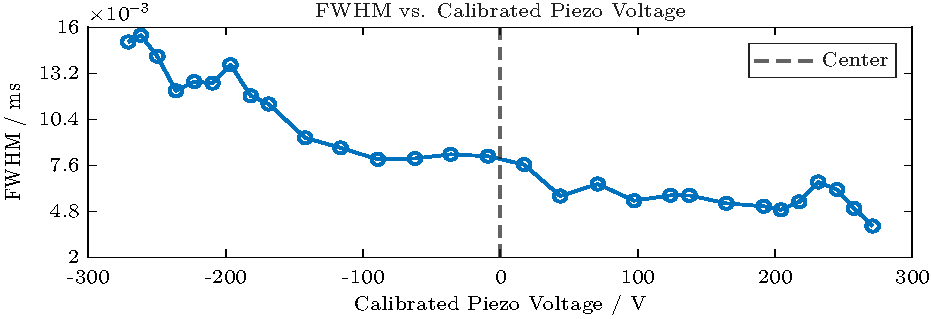
\includegraphics[width=\textwidth]{Figure_3.pdf}
        \caption{Zoomed-in view of Peak 1.}
        \label{fig:peak1}
    \end{subfigure}
    \hfill
    \begin{subfigure}[t]{0.48\textwidth}
        \centering
        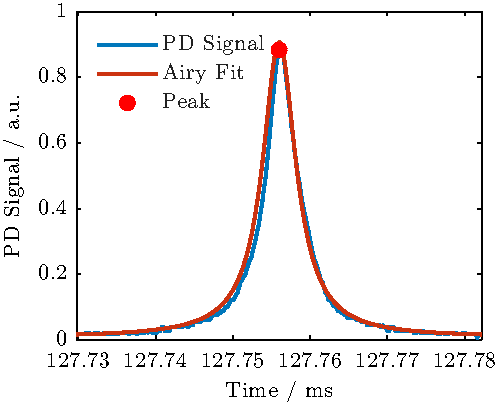
\includegraphics[width=\textwidth]{Figure_4.pdf}
        \caption{Zoomed-in view of Peak 2.}
        \label{fig:peak2}
    \end{subfigure}
    \caption{Zoomed-in views of the detected peaks in the selected region.}
\end{figure}
